\chapter{Studio di funzione}
\texttt{In analisi matematica la locuzione studio di funzione indica 
	l'applicazione pratica dei teoremi e delle tecniche del calcolo 
	infinitesimale nello specifico caso di una funzione di cui è nota 
	l'espressione analitica. Lo studio di funzione è utile per ricavare 
	esplicitamente le informazioni che descrivono il comportamento di una 
	funzione nel suo dominio. Spesso, le informazioni ottenute mediante uno 
	studio di funzione sono sufficienti per poter tracciare, anche a mano, un 
	grafico qualitativo della funzione studiata e che in genere, per funzioni a 
	valori reali di una variabile reale, viene rappresentato su un piano 
	cartesiano, anche se in taluni casi potrebbe essere più semplice ricorrere 
	un sistema di coordinate differente. In genere, con "studio di funzione" ci 
	si riferisce implicitamente al solo e specifico caso delle funzioni reali di
	una sola variabile reale, ma con le opportune modifiche è comunque possibile 
	adattare le considerazioni seguenti anche al caso delle funzioni di più
	variabili reali, nonché anche per le funzioni di una o più variabili 
	complesse.}
\begin{center}
	By \href{https://it.wikipedia.org/wiki/Studio_di_funzione}{Wikipedia}
\end{center}

\section{Grafica delle funzioni elementari}
\subsection{Funzione lineare $y=mx+qm, q\in R$}
\begin{figure}[!ht]
	\centering
	\begin{tikzpicture}
		\node[] (pic) at (0,0) {\includegraphics[height=8cm]{img/funzione
		lineare.pdf}};
	\end{tikzpicture}
	\caption{Grafico di Funzione lineare $y=mx+qm, q\in R$}
\end{figure}
$C.E. \equiv R\text{ Non Limitata}$
\subsection{Funzione valore assoluto $y=|x|$}
\begin{figure}[!ht]
	\centering
	\begin{tikzpicture}
		\node[] (pic) at (0,0) {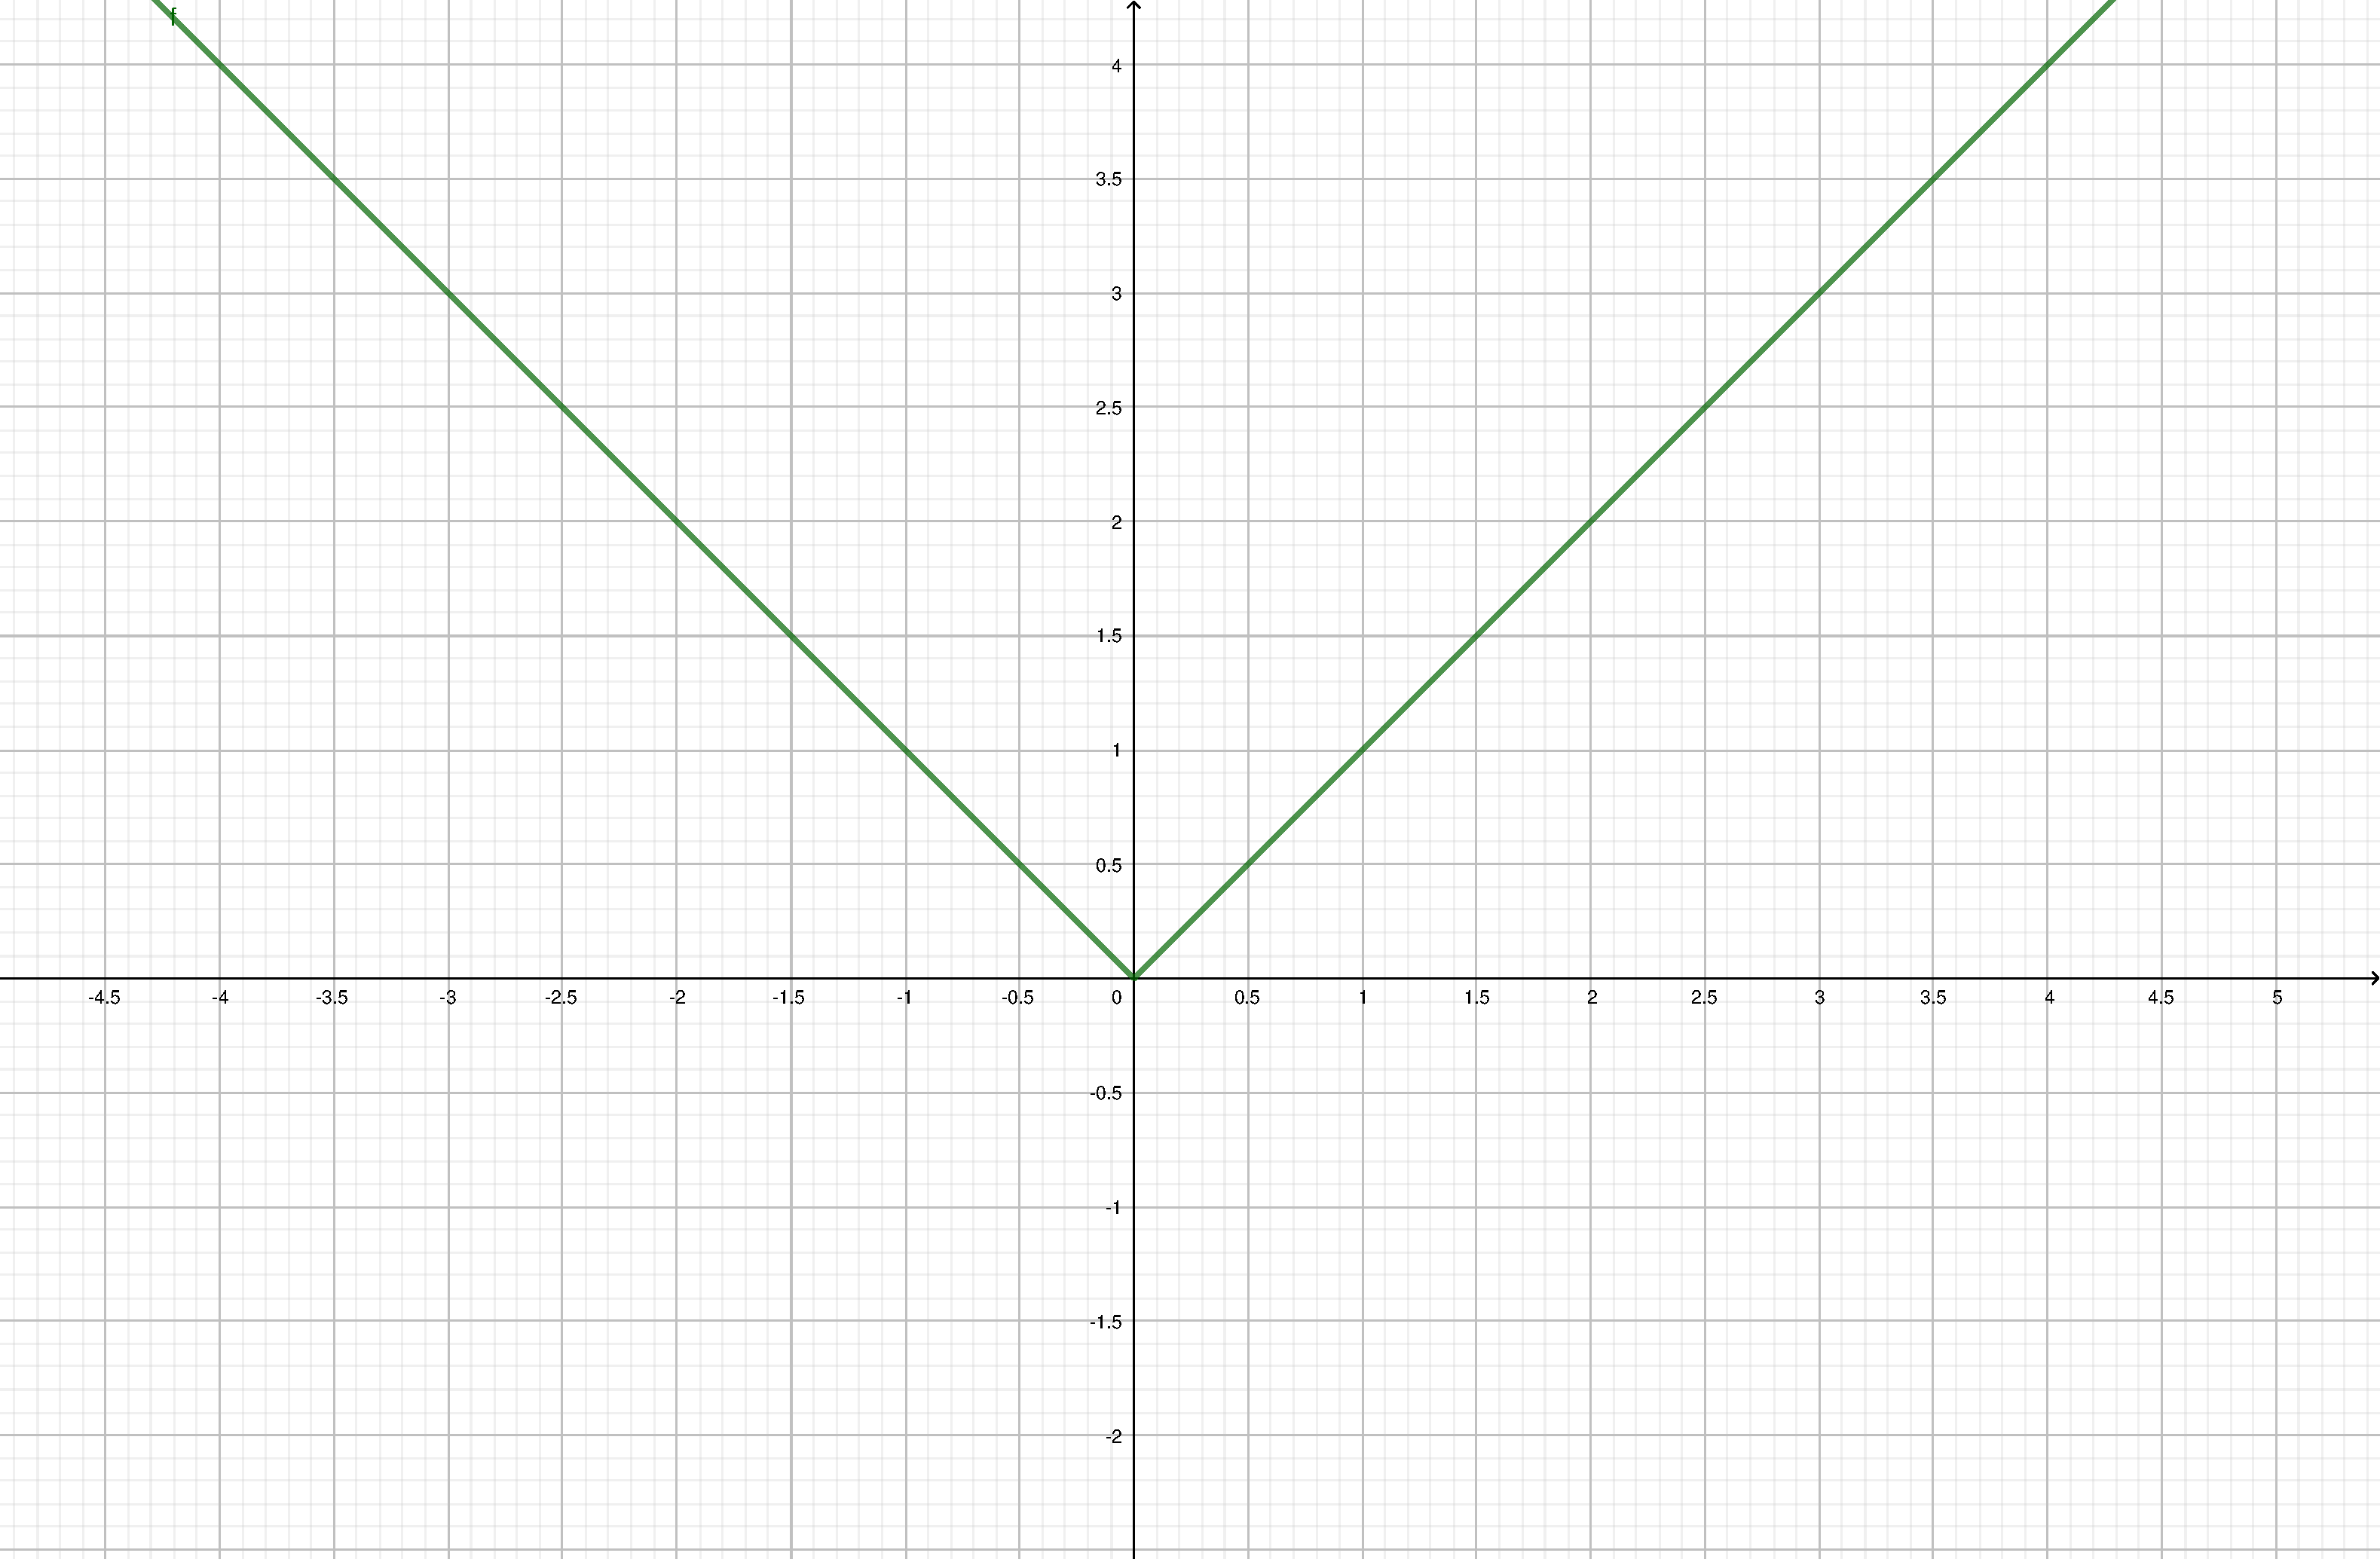
\includegraphics[height=8cm]{img/funzione valore assoluto.pdf}};
	\end{tikzpicture}
	\caption{Grafico di Funzione valore assoluto $y=|x|$}
\end{figure}
$C.E. \equiv R\text{ Limitata inferiormente in } x=0$\\
$|x|=\begin{cases}
	x&x\geq0\\
	-x& x<0
\end{cases}$
\subsection{Funzione potenza $y=x^n,n\in N, pari$}
\begin{figure}[!ht]
	\centering
	\begin{tikzpicture}
		\node[] (pic) at (0,0) {\includegraphics[height=8cm]{img/funzione
		potenziale x^n.pdf}};
	\end{tikzpicture}
	\caption{Grafico di Funzione potenza $y=x^n,n\in N, pari$}
\end{figure}\newpage
\subsection{Funzione potenza $y=x^\alpha,\alpha \in R$ (\textit{ma non
razionale})}
\begin{figure}[!ht]
	\centering
	\begin{tikzpicture}
		\node[] (pic) at (0,0) {\includegraphics[height=8cm]{img/funzione
		potenziale x^a.pdf}};
	\end{tikzpicture}
	\caption{Grafico di Funzione potenza $y=x^\alpha,\alpha \in R$ (\textit{ma non
razionale})}
\end{figure}
$C.E.:\{x\in R: x\geq 0\}$ Limitata inferiormente da $x=0$ non limitata
superiormente Strettamente crescente
\subsection{Funzione potenziale $y=x^{\frac{m}{n}},m, n\in Z$}
\begin{figure}[!ht]
	\centering
	\begin{tikzpicture}
		\node[] (pic) at (0,0) {\includegraphics[height=8cm]{img/funzione
		potenziale fratta.pdf}};
	\end{tikzpicture}
	\caption{Grafico di Funzione potenza $y=x^\alpha,\alpha \in R$ (\textit{ma non
razionale})}
\end{figure}
\subsection{Funzione logaritmo $y=\log_a{x}$}
\begin{figure}[!ht]
	\centering
	\begin{tikzpicture}
		\node[] (pic) at (0,0) {\includegraphics[height=8cm]{img/funzione
		logaritmica.pdf}};
	\end{tikzpicture}
	\caption{Funzione logaritmo $y=\log_a{x}$}
\end{figure}
$C.E.\equiv x>0$ Non limitata, strettamente crescente se $a>1$, Strettamente
decrescente se $0<a<1$.\newpage
\subsection{Le coniche: la circonferenza}
\begin{figure}[!ht]
	\centering
	\begin{tikzpicture}
		\node[] (pic) at (0,0) {\includegraphics[height=8cm]{img/le coniche
		circonferenze.pdf}};
	\end{tikzpicture}
	\caption{Le coniche: la circonferenza}
\end{figure}\newpage
\subsection{Le coniche: l'ellisse}
\begin{figure}[!ht]
	\centering
	\begin{tikzpicture}
		\node[] (pic) at (0,0) {\includegraphics[height=8cm]{img/le coniche
		ellisse.pdf}};
	\end{tikzpicture}
	\caption{Le coniche: l'ellisse}
\end{figure}
\subsection{Le coniche: iperbole}
\begin{figure}[!ht]
	\centering
	\begin{tikzpicture}
		\node[] (pic) at (0,0) {\includegraphics[height=8cm]{img/le coniche
		iperbole.pdf}};
	\end{tikzpicture}
	\caption{Le coniche: iperbole}
\end{figure}\newpage
\subsection{Le coniche: iperbole equilattera}
\begin{figure}[!ht]
	\centering
	\begin{tikzpicture}
		\node[] (pic) at (0,0) {\includegraphics[height=8cm]{img/le coniche
		iperbole equilattera.pdf}};
	\end{tikzpicture}
	\caption{Le coniche: iperbole equilattera}
\end{figure}
\subsection{Le coniche: parabola}
\begin{figure}[!ht]
	\centering
	\begin{tikzpicture}
		\node[] (pic) at (0,0) {\includegraphics[height=8cm]{img/le coniche
		parabola.pdf}};
	\end{tikzpicture}
	\caption{Le coniche: parabola}
\end{figure}\newpage
\subsection{Le funzioni trigonometriche}
Funzioni trigonometriche elementati:
$y=\sin x, y=cos x, y=\tan x, y=\cot x$\\
\textit{Relazioni fondamentali:} $(\sin x)^2+(\cos x)^2=1$, $\tan x=\frac{\sin
x}{\cos x}$, $\cot x=\frac{\cos x}{\sin x}$
\begin{figure}[!ht]
	\centering
	\begin{tikzpicture}
		\node[] (pic) at (0,0) {\includegraphics[height=8cm]{img/funzioni
		trigonometriche.pdf}};
	\end{tikzpicture}
	\caption{Le funzioni trigonometriche}
\end{figure}
\subsubsection{Funzione $\sin x$}
\begin{figure}[!ht]
	\centering
	\begin{tikzpicture}
		\node[] (pic) at (0,0) {\includegraphics[height=8cm]{img/funzione
		sin.pdf}};
	\end{tikzpicture}
	\caption{Funzione $\sin x$}
\end{figure}\newpage
\subsubsection{Funzione $\cos x$}
\begin{figure}[!ht]
	\centering
	\begin{tikzpicture}
		\node[] (pic) at (0,0) {\includegraphics[height=8cm]{img/funzione
		cos.pdf}};
	\end{tikzpicture}
	\caption{Funzione $\cos x$}
\end{figure}
\subsubsection{Funzione $\tan x$}
\begin{figure}[!ht]
	\centering
	\begin{tikzpicture}
		\node[] (pic) at (0,0) {\includegraphics[height=8cm]{img/funzione
		tg.pdf}};
	\end{tikzpicture}
	\caption{Funzione $\tan x$}
\end{figure}\newpage
\subsubsection{Funzione $\cot x$}
\begin{figure}[!ht]
	\centering
	\begin{tikzpicture}
		\node[] (pic) at (0,0) {\includegraphics[height=8cm]{img/funzione
		ctg.pdf}};
	\end{tikzpicture}
	\caption{Funzione $\cot x$}
\end{figure}
\subsection{Le funzioni trigonometriche inverse}
\subsubsection{Funzione $\arcsin x$}
\begin{figure}[!ht]
	\centering
	\begin{tikzpicture}
		\node[] (pic) at (0,0) {\includegraphics[height=8cm]{img/funzione
		arcsin.pdf}};
	\end{tikzpicture}
	\caption{Funzione $\arcsin x$}
\end{figure}\newpage
\subsubsection{Funzione $\arccos x$}
\begin{figure}[!ht]
	\centering
	\begin{tikzpicture}
		\node[] (pic) at (0,0) {\includegraphics[height=8cm]{img/funzione
		arccos.pdf}};
	\end{tikzpicture}
	\caption{Funzione $\arccos x$}
\end{figure}
\subsubsection{Funzione $\arctan x$}
\begin{figure}[!ht]
	\centering
	\begin{tikzpicture}
		\node[] (pic) at (0,0) {\includegraphics[height=8cm]{img/funzione
		arctg.pdf}};
	\end{tikzpicture}
	\caption{Funzione $\arctan x$}
\end{figure}\newpage
\subsubsection{Operazione sul grafico: traslazione della asse X}
\begin{figure}[!ht]
	\centering
	\begin{tikzpicture}
		\node[] (pic) at (0,0) {\includegraphics[height=8cm]{img/operazione sul
		grafico traslazione della asse x.pdf}};
	\end{tikzpicture}
	\caption{Operazione sul grafico: traslazione della asse X}
\end{figure}
\subsubsection{Operazione sul grafico: traslazione della asse Y}
\begin{figure}[!ht]
	\centering
	\begin{tikzpicture}
		\node[] (pic) at (0,0) {\includegraphics[height=8cm]{img/operazione sul
		grafico traslazione della asse y.pdf}};
	\end{tikzpicture}
	\caption{Operazione sul grafico: traslazione della asse Y}
\end{figure}\newpage
\subsubsection{Operazione sul grafico: contrazione e dilatazione in direzione verticale}
\begin{figure}[!ht]
	\centering
	\begin{tikzpicture}
		\node[] (pic) at (0,0) {\includegraphics[height=8cm]{img/contrazione e
		dilatazione in direzione verticale.pdf}};
	\end{tikzpicture}
	\caption{Operazione sul grafico: contrazione e dilatazione in direzione verticale}
\end{figure}
\subsubsection{Operazione sul grafico: contrazione e dilatazione in direzione
orizzontale}
\begin{figure}[!ht]
	\centering
	\begin{tikzpicture}
		\node[] (pic) at (0,0) {\includegraphics[height=8cm]{img/compressione e
		dilatazione in direzione orizzontale.pdf}};
	\end{tikzpicture}
	\caption{Operazione sul grafico: contrazione e dilatazione in direzione
	orizzontale}
\end{figure}\newpage
\subsubsection{Operazione sul grafico: $y=|f(x)|$}
\begin{figure}[!ht]
	\centering
	\begin{tikzpicture}
		\node[] (pic) at (0,0) {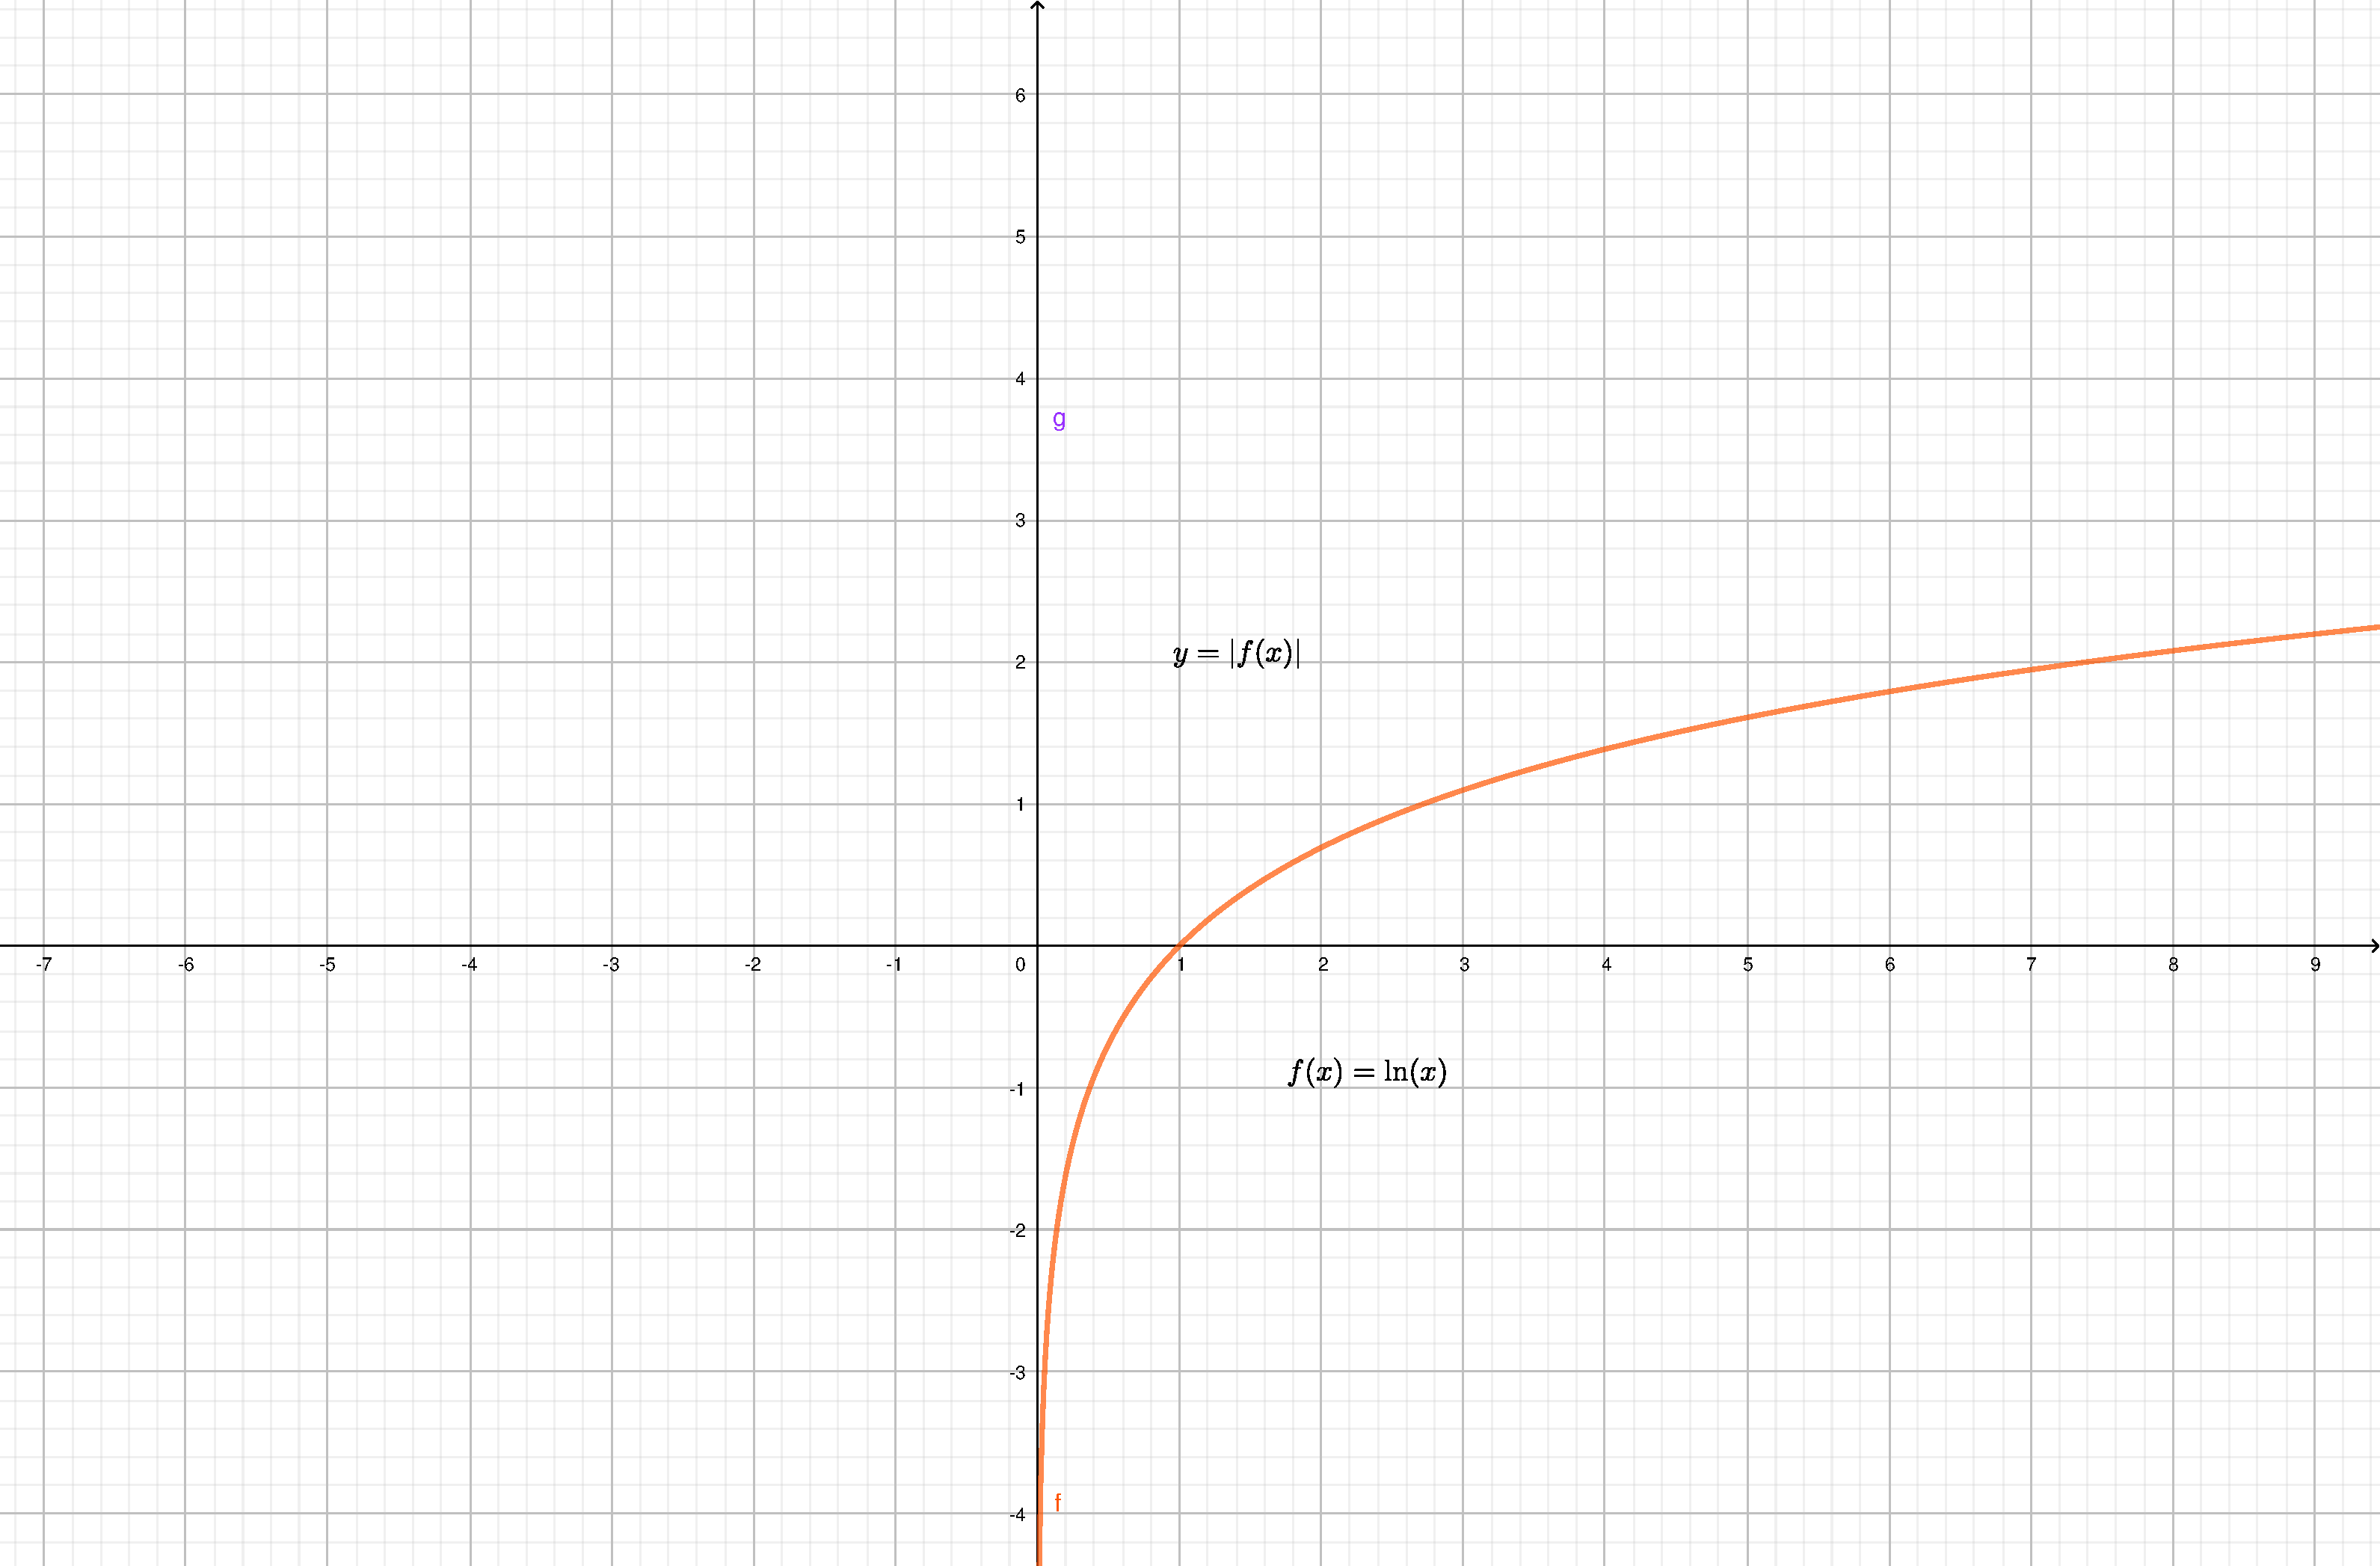
\includegraphics[height=8cm]{img/y=_lnx_.pdf}};
	\end{tikzpicture}
	\caption{Operazione sul grafico: $y=|f(x)|$}
\end{figure}

% passaggio ai limiti

\section{Limiti}
\begin{figure}[!ht]
	\centering
	\begin{tikzpicture}
		\node[] (pic) at (0,0) {\includegraphics[height=8cm]{img/esempio limite
		di funzione.pdf}};
	\end{tikzpicture}
	\begin{tabular}{|l|l|}
		\hline
		x&f(x)\\\hline\hline
		0,1& 0,998\\
		0,001&0,999\\\hline
	\end{tabular}
	$C.E.=R\textbackslash{}\{0\}$
	\caption{Esempio limite di funzione}
\end{figure}
Il limite di una funzione è un operazione, o meglio un operatore, che permette
di studiare il comportamento di una funzione nell'intorno di un punto $x_0$.\\
\textit{Mediamente il limite è possibile stabilire a quale valore tende la
funzione man mano che i valori della variabile si approssimano al punto $x_0$}.
\begin{figure}[!ht]
	\centering
	\begin{tikzpicture}
		\node[] (pic) at (0,0) {\includegraphics[height=8cm]{img/esempio di
		limite di una funzione.pdf}};
	\end{tikzpicture}
	\caption{Esempio di limite di una funzione}
\end{figure}
\subsection{Limite di una funzione}
Sia $f(x)$ definita in $A\in R$, e sia $x_0$ un punto di accumulazione per A.
Si dice che $f(x)$ ha limite $l$ per $x$ che tende a $x_0$, se $V\varepsilon
>0 \exists \delta_\varepsilon > 0: |f(x)-l|=\varepsilon\Rightarrow x\in
I(x_0,\delta_\varepsilon) \text{ escluso al più } x_0 \text{ cioè }
|x-x_0|<\delta_\varepsilon$
\begin{itemize}
	\item $l-\varepsilon < f(x) < l+\varepsilon$
	\item $x_0-\varepsilon < x<x_0+\delta_\varepsilon$
\end{itemize}
\subsubsection{In simboli}
$\lim_{x\to x_0} f(x)=l \text{   } f(x)\xrightarrow{x\to x_0} l$ 
\subsection{Definizione di Limite destro}
$l_1$ si definisce \textit{limite 
destro} di $f(x)$ per x che tende a $x_0^+$: $\lim_{x\to x_0^+ f(x)=l_1}$\\
se $\forall \varepsilon > 0 \exists \delta_\varepsilon>0 :
|f(x)-l_1|<\varepsilon\Rightarrow x_0<x<x_0+\delta_\varepsilon \text{ cioè }
x\in(x_0,x_0+\delta_\varepsilon)$
\subsection{Definizione di limite sinistro ``da sinistra''}
$l_2$ si definisce \textit{limite sinistro} di $f(x)$ per \textit{x} che tende
a $x^-_0$: $\lim_{x\to x_0^-}f(x)=l^2$ se $\forall \varepsilon>0 \exists
\delta_\varepsilon>0: |f(x)-l_2|<\varepsilon\Rightarrow
x_0-\delta_\varepsilon<x<x_0$ cioè $x\in(x_0-\delta_\varepsilon,x_0)$
\subsection{Teorema d'unicità del limite ``da destra''}
Se $\lim_{x\to x_0} f(x)=l\Rightarrow \text{l è unico}$\\
Dimostrazione. Per assurdo: supponiamo che $\exists l_1,l_2: l_1 \neq l_2$
con $l_1=lim_{x\to x_0}f(x)$ in $I(x_0,\delta_{1\varepsilon})$, $l_2=lim_{x\to
x_0}f(x)$ in $I(x_0,\delta_{2\varepsilon})$\\
Fissato $\varepsilon=\frac{|l_1-l_2|}{2}$\\
$2\varepsilon=|l_1-l_2|=|l_1-f(x)+f(x)-l_2|\leq|f(x)-l_2|+|f(x)-l_2|<2\varepsilon$
in $I(x_0,\delta_{\varepsilon})$,
$\delta_{\varepsilon}=min(\delta_{1\varepsilon},\delta_{2\varepsilon})$
Assurdo! $\Rightarrow l_1=l_2$
\subsubsection{Esempi}
\begin{tabular}{lc}
	$y=\frac{|x|}{x}$ & $C.E. = R\textbackslash \{0\}$\\
	$\lim_{x\to 0^+}\frac{|x|}{x}=1$&\multirow{2}{*}{$\nexists \text{ limitate}$} \\
	$\lim_{x\to 0^-}\frac{|x|}{x}=-1$&\\
\end{tabular}
\paragraph{Definizione} Sia $f(x)$ definita in $A \in R$, e sia $x_0$ un punto
di accumulazione per A. Si dice che $f(x)$ ha limite $+\infty$ per x che tende
a $x_0$, se $\forall M>0,\exists \delta_M>0:\forall x \in
I(x_0,\delta_m)\Rightarrow f(x)>M$
\begin{center}
	\begin{tabular}{|l|}
		\hline
		$\lim_{x\to x_0}f(x)=+\infty$\\\hline
	\end{tabular}
\end{center}
\paragraph{Definizione} Sia $f(x)$ definita in $A\in R$, e sia $x_0$ un punto
di accumulazione per A. Si dice che $f(x)$ ha limite $-\infty$ per $x$ che
tende a $x_0$, se $\forall M>0, \exists \delta_M>0:\forall x \in
I(x_0,\delta_m)$\\
risulta $f(x)<-M$.
\begin{center}
	\begin{tabular}{|l|}
		\hline
		$\lim_{x\to x_0}f(x)=-\infty$\\\hline
	\end{tabular}
\end{center}
\paragraph{Definizione di Asintoto verticale}
Se $\boxed{\lim_{x\to x_0}f(x)=\infty}$ allora la retta verticale $\boxed{x=x_0}$
si chiama asintoto verticale
\begin{figure}[!ht]
	\centering
	\begin{tikzpicture}
		\node[] (pic) at (0,0) {\includegraphics[height=8cm]{img/asintoto
		verticale.pdf}};
	\end{tikzpicture}
	\caption{Asintoto verticale}
\end{figure}\\
Sia $f(x)$ definita in $A\in R$, si dice che $f(x)$ ha limite $l$, per $x$ che
tende a $+\infty$, se: $\forall_\varepsilon>0, \exists K_\varepsilon >0:\forall
x \in I (K_\varepsilon, +\infty)$ risulta $|f(x)-l|<\varepsilon$
\begin{equation*}
	\boxed{\lim_{x\to+\infty}f(x)=l}
\end{equation*}
\newpage
\paragraph{Definizione di Asintoto orizzontale} Se \begin{tabular}{|l|}
	\hline
	$\lim_{x\to \infty}f(x)=l$\\\hline
\end{tabular} Allora la retta orizzontale $\boxed{y=l}$ si chiama Asintoto orizzontale
\begin{figure}[!ht]
	\centering
	\begin{tikzpicture}
		\node[] (pic) at (0,0) {\includegraphics[height=8cm]{img/asintoto
		orizzontale.pdf}};
	\end{tikzpicture}
	\caption{Asintoto orizzontale}
\end{figure}\\
Sia $f(x)$ definita in $A \in R$, si dice che $f(x)$ ha limite $+\infty$, per x
che tende a $+\infty$, se: $\forall M>0, \exists K_M >0: \forall x \in (K_M,
+\infty)$ risulta $f(x)\in (M,+\infty)$ \begin{tabular}{|l|}
	$\lim_{x\to +\infty}f(x) = +\infty$
\end{tabular}
\subsection{Teorema (\texttt{\color{red} algebra dei limiti})}
Se:
\begin{itemize}
	\item $\lim_{x\to x_0} f(x)=l_1$ $\lim_{x\to x_0} g(x) = l_2$
	\item $\lim_{x\to x_0} f(x)\pm g(x)=l_1\pm l_2$
	\item $\lim_{x\to x_0} f(x)*g(x)=l_1*l_2$
	\item $\lim_{x\to x_0} \frac{f(x)}{g(x)}=\frac{l_1}{l_2}, g(x), l_2\neq 0$

\end{itemize}
\subsection{Convenzioni con $\infty$}
\begin{itemize}
	\item $\forall a >0, a\pm \infty=\pm \infty$
	\item $+\infty+\infty=+\infty$
	\item $-\infty-\infty=-\infty$
	\item $\forall a> 0, a*(\pm \infty)=\pm \infty$
	\item $\forall b< 0, b*(\pm \infty)=\mp \infty$
	\item $(\pm\infty)*(\pm \infty)=+\infty$
	\item $(\pm\infty)*(\mp \infty)=-\infty$

\end{itemize}
\subsubsection{Convenzioni con $\infty$}
$\frac{a}{\infty}=0$ $\frac{a}{0}=\infty$

\subsection{Forme indeterminate}
\begin{tabular}{|llllll|}
	\hline
	$+\infty-\infty$&$\frac{\infty}{\infty}$&$\frac{0}{0}$&$1^\infty$&$e^{+\infty*0}$&$0-\infty$\\
	\hline
\end{tabular}
\begin{itemize}
	\item $a^{+\infty}=\begin{cases}
			+\infty,&a>1\\
			0,&0<a<1
	\end{cases}$
	\item $a^{-\infty}=\begin{cases}
			0,&a>1\\
			+\infty,&0<a<1
	\end{cases}$
\end{itemize}
\subsection{Teorema del confronto}
Siano $f(x),f_1(x),f_2(x)$ tre funzioni definite in $A\subseteq R$ sia $x_0$ un
punto di accumulazione per A e $f_1(x)\leq f(x) \leq f_2(x)$ se $\lim_{x\to
x_0}f_1(x)=\lim_{x\to x_0} f_2(x)=l$ allora $\lim_{x\to x_0} f(x)=l$
\subsubsection{Dimostrazione}
Se $\lim_{x\to x_0} f_1(x)=\lim_{x\to x_0} f_2(x)=l$ allora per definizione di
limite:
\begin{itemize}
	\item $\exists \delta_1:|f_1(x)-l|<\varepsilon$ $\forall x \in I(x_0,\delta_1)$
	\item $\exists \delta_2:|f_2(x)-l|<\varepsilon$ $\forall x \in
		I(x_0,\delta_2)$
\end{itemize}
\begin{center}
	$\Rightarrow l-\varepsilon < f_1(x) \leq f(x)\leq f_2(x) < l+ \varepsilon$
\end{center}
$\forall x \in I(x_0,\delta_2), \delta = \min (\delta_1,\delta_2)$
\subsubsection{Casi particolari di $\lim_{x\to x_0} f(x)*g(x)$}
\paragraph{Teorema}
Se $\lim_{x\to x_0} f(x)=x$; $|g(x)|\leq M$ per $x\in I(x_0,\delta)\Rightarrow
\lim_{x\to x_0}f(x)*g(x)=0$
\subparagraph{Esempio} $\lim_{x\to x_0}x*\sin\frac{1}{x}=0$
\subsection{Limite di \texttt{funzione composta}}
Siano $g:A\to B:B\to R:$ $\lim_{x\to x_0}g(x)=y_0$ e $\lim_{y\to y_0}f(y)=l$
con $l=f(y_0)$ (\textit{se f è continua})\\
$\Rightarrow$\begin{tabular}{|l|}
	\hline$\lim_{x\to x_0}f[g(x)]=l$\\\hline
\end{tabular}
\subsection{Limiti Notevoli}
\begin{multicols}{2}
	\begin{itemize}
		\item \begin{tabular}{|l|}
				\hline
				$\lim_{x\to x_0}\frac{\sin (x)}{x}=1$\\\hline
		\end{tabular}
		\item \begin{tabular}{|l|}
				\hline
				$\lim_{x\to x_0}\frac{\tan (x)}{x}=1$\\\hline
		\end{tabular}
		\item \begin{tabular}{|l|}
				\hline
				$\lim_{x\to x_0}\frac{1-\cos (x)}{x}=\frac{1}{2}$\\\hline
		\end{tabular}
		\item \begin{tabular}{|l|}
				\hline
				$\lim_{x\to x_0}(1+\frac{1)}{x})=e$\\\hline
		\end{tabular}
		\item \begin{tabular}{|l|}
				\hline
				$\lim_{x\to x_0}\frac{\log_a (1+x)}{x}=log_ae$\\\hline
		\end{tabular}
		\item \begin{tabular}{|l|}
				\hline
				$\lim_{x\to x_0}\frac{a^x-1}{x}=\log_ea$\\\hline
		\end{tabular}
	\end{itemize}
\end{multicols}
\paragraph{Esempi}
\begin{multicols}{2}
	\begin{enumerate}
		\item $\lim_{x\to x_0^+}xe^x+e^{-\frac{1}{x}}=0$
		\item $\lim_{x\to x_0^-}xe^x+e^{-\frac{1}{x}}=\infty$
		\item $\lim_{x\to x_0}\frac{1-\cos (x)}{x^2}=\lim_{x\to
			x_0}\frac{(1-\cos (x))(1+\cos (x))}{x^2(1+\cos x)}=\frac{1}{2}$
		\item $\lim_{x\to +\infty}\frac{1}{x}+\arctan{x}=\frac{\pi}{2}$
	\end{enumerate}
\end{multicols}
\begin{figure}[!ht]
	\centering
	\begin{tikzpicture}
		\node[] (pic) at (0,0) {\includegraphics[height=8cm]{img/esempio studio
		di funzione 2.pdf}};
	\end{tikzpicture}
	\caption{Esempio di limite notevole di una funzione}
\end{figure}

\subsection{Infinitesimi e infiniti}
\paragraph{Definizione}
Una funzione $f(x)$ su dice \underline{infinitesima} per $x\to x_0$ (per $x\to \infty$), $x_0$ punto di accumulazione per il dominio di $f(x)$, se: $\lim_{x\to x_0}f(x)=0$ (oppure $lim_{x\to \infty}f(x)=0$).
\subsubsection{Esempi}
\begin{itemize}
	\item $y=e^x$ è un infinitesimo per $x\to -\infty$
	\item $y=\ln{x}$ è un infinitesimo per $x\to 1$
	\item $y=\sin{x}$ è un infinitesimo per $x\to 0$ (ma anche per $x\to \pi,2\pi$, etc.)
	\item $y=\ln{1+x}$ è un infinitesimo per $x\to 1$ 
\end{itemize}
\subsubsection{Ordine di infinitesimo}
Siano $f(x)$ e $g(x)$ infinitesimi per $x\to{x_0}$ (o per $x\to \infty$), con $g(x)\neq 0$. Se $\exists\alpha R+$ e $l\in R$, $l\neq 0$ tale che\\
$\lim_{x\to{x_0}}=\frac{f(x)}{[g(x)]^\alpha}=l$ (oppure $\lim_{x\to{\infty}}=\frac{f(x)}{[g(x)]^\alpha}=l$)\\
Allora, si dice che per $x\to x_0$ (o per $x\to \infty$), $f(x)$ è un infinitesimo di ordine $\alpha$ rispetto all'infinitesimo campione $g(x)$.
\paragraph{Esempi}
\begin{itemize}
	\item $y=\sin{x}$ è un infinitesimo per $x\to 0$ di ordine 1 rispetto all'infinitesimo campione $g(x)=x$, infatti, $\lim_{x\to 0}=\frac{\sin{x}}{x^\alpha}=1$ solo se $\alpha = 1$
	\item $y=\tan^2x$ è un infinitesimo di ordine 2 rispetto ad x, per $x\to 0$
	\item $ord(l-\cos{x})=2$ rispetto ad $x$ per $x\to 0$
\end{itemize}
\subsubsection{Confronto tra infinitesimi}
Siano $f(x)$ e $g(x)$ infinitesime per $x\to x_{0}$,\\
$\lim_{x\to x_0}\frac{f(x)}{g(x)}=
\begin{cases}
l\neq 0&ord(f)=ord(g)\\
\pm \infty&ord(f)<ord(g)\\
0&ord(f)>ord(g)\\
	\text{non esiste,} & \text{f e g non confrontabile} \\ 
\end{cases}
$\\
Stesso risultato se $f(x)$ e $g(x)$ sono infinitesime per $x\to \infty$. Utilizzando il confronto tra infinitesimi nel calcolo dei limiti del tipo $\lim_{x\to x_0}\frac{f_1+f_2}{g_1+g_2}$, dove $f_1,f_2,g_1,g_2$ sono funzioni infinitesime per $x\to x_0$, si possono {\color{blue} \em trascurare gli infinitesimi di ordine maggiore} (analogo discorso per funzioni infinitesime $x\to \infty$).
\subparagraph{esempio}
$\lim_{x\to 0}\frac{x^2+x^3+2\tan{x}}{(e^x-1)^2+\sin{x}}=\lim_{x\to 0}\frac{2\tan x}{\sin x}=2$
\paragraph{Definizione di funzioni asintotiche}
Si dice che due funzioni $f,g$ sono asintotiche per $x\to x_0$ se $\lim_{x\to x_0}\frac{f(x)}{g(x)}=1$ e si scrive $f\sim g$ per $x\to x_0$
\subparagraph{esempi}
\begin{itemize}
	\item $\sin x\sim x$ per $x\to 0$
	\item $\ln(1+x)\sim x$ per $x\to 0$
	\item $e^x-1\sim x$ per $x\to 0$ 
\end{itemize}
\paragraph{Definizione di funzioni infinite}
Una funzione $f(x)$ si dice \textit{infinita} per $x\to x_0$ (o per $x \to \infty$) , $x_0$ punto di accumulazione per il dominio di $f(x)$, (o per $x\to \infty$) se:
\begin {center}
	$\lim_{x\to x_0}f(x)=\infty$ (oppure $\lim_{x\to \infty}f(x)=\infty$)
\end{center}
\subparagraph{Esempi}
\begin{itemize}
	\item $y=e^x$ è un infinito per $x\to +\infty$
	\item $y=\ln{x}$ è un infinito per $x\to 0^+$
	\item $y=x^2+x$ è un infinito per $x\to \infty$
\end{itemize}
\subparagraph{Regole aritmetiche}
Siano $f(x)=o(x^\alpha)$ (si legge <<o piccolo di>>) e $g(x)=o(x^\beta)$ due funzioni \textit{infinitesime} rispettivamente di ordine $\alpha$ e $\beta$ per $x \to 0$ Allora si ha
\begin{itemize}
	\item $cf(x))o(x^\alpha)$, $\forall c \in R$
	\item $x^\lambda f(x)=o(x^{\lambda+\alpha})$
	\item $f(x)g(x)=o(x^{\alpha+\beta})$
	\item $f(x)+g(x)=o(x^y)$, $\gamma=min(\alpha,\beta)$
\end{itemize}
\paragraph{Ordine di infinito}
Siamo $f(x)$ e $g(x)$ infiniti per $x\to x_0$ (o per $x$), con $g\neq 0$. Se $\exists\alpha\in R+$ e $l\in R$, $l\neq 0$ tale che\\
$\lim_{x\to x_0}\frac{f(x)}{[g(x)]^2}=l$ (o $\lim_{x\to \infty}\frac{f(x)}{[g(x)]^\alpha}=l$)\\
Allora, per $x\to x_0$ (o per $x\to \infty$), $f(x)$ è un infinito di ordine $\alpha$ rispetto all'infinito compone $g(x)$.
\subparagraph{Esempi}
\begin{itemize}
	\item $ord(\sqrt{x})=\frac{1}{2}$ rispetto ad $x$ per $x\to +\infty$
	\item $ord(\frac{1}{\sin x})=1$ rispetto ad $\frac{1}{x}$ per $x\to 0$
	\item $ord(\frac{1}{e^x-1})=1$ rispetto ad $\frac{1}{x}$ per $x\to 0$
\end{itemize}
\subparagraph{Cofronto tra infiniti}
Siamo $f(x)$ e $g(x)$ infiniti per $x\to x_0$\\
$\lim_{x\to x_0}\frac{f(x)}{g(x)}=\begin{cases}
l\neq 0&ord(f)=ord(g)\\
\pm \infty&ord(f)>ord(g)\\
0&ord(f)<ord(g)\\
	\text{non esiste,} & \text{f e g non confrontabile} \\ 
\end{cases}
$\\
Stesso risultato se $f(x)$ e $g(x)$ sono infinite per $x \to \infty$. Utilizzando il confronto tra infiniti nel calcolo dei limiti del tipo $\lim_{x\to x_0}\frac{f_1+f_2}{g_1+g_2}$, deve $f_1,f_2,g_1,g_2$ sono funzioni infinite per $x\to x_0$, si possono {\color{red}trascurare gli \underline{infiniti} di ordine minore} (analogo discorso per funzione infinito $x\to \infty$).
\subparagraph{Esempio}
$\lim_{x\to +\infty}\frac{x^2+x^3+3\sqrt{x}}{x^2(2x-1)+\sqrt{3x}}=\lim_{x\to +\infty}\frac{x^3}{2x^3}=\frac{1}{2}$.
\paragraph{Gerarchia degli infiniti}
Per $x\to +\infty$ si ha $(\log_\alpha x)^\alpha<<x^\beta<<b^x$, con $\alpha,\beta>0,a,b>1$ Non sempre è possibile calcolare l'ordine di infinito (o di infinitesimo) rispetto alla funzione campione usuale.\\
\subparagraph{Esempio}
$\lim_{x\to +\infty}\frac{a^x}{x^a}=+\infty, \forall \alpha>0, a>1$, $\lim_{x\to +\infty}\frac{(\log_a x)^\beta}{x^a}=+\infty, \forall \alpha, \beta>0, a>1$
\subparagraph{Regole aritmetiche}
Siano $f(x)$ e $g(x)$ due funzioni \emph{infinite} di ordine rispettivamente $\alpha$ e $\beta$. Allora si ha
\begin{itemize}
	\item $ord(f(x)+g(x))=\max{\alpha,\beta}$
	\item $ord(f(x)*g(x))=\alpha+\beta$
	\item $ord((f(x))^\gamma)=\alpha\gamma$
\end{itemize}
\subsection{Funzioni continue}
Una funzione continua è una funzione che, intuitivamente, fa corrispondere ad elementi sufficientemente vicini del dominio elementi arbitrariamente vicini del codominio.
\paragraph{Definizione} Una funzione $f(x)$ è continua in $x_0$, se: $l_1=\lim_{x\to x^+_0}=\lim_{x\to x_0}f(x)=l_2=\lim_{x\to x_0}f(x)=f(x_0)$ ossia $\forall\in>0\exists \delta_\mathcal{E} > 0$: $|f(x)-f(x_0)|<\mathcal{E}$ $\forall_x\in I(x_0,\delta_\mathcal{E})$ $(l=f(x_0))$
\subsubsection{Teorema della permanenza del segno}
Sia f(x) definita almeno in un intorno di $x_0$ e continua in $x_0$. Se $f(x_0)>0$ allora $\exists \delta >0 : f(x) >0 \forall x\in (x_0-\delta ,x_0+\delta{})$
\subsubsection{Teorema degli zeri}
Sia $f(x)$ continua in $[a,b]$ $f(a)*f(b)<0$ allora $\exists x_0 \in (a,b): f(x_0)=0$. Se $f$ è anche strettamente monotona, lo zero è unico.
\paragraph{Teorema dell'esistenza dei valori intermedi (\textit{conseguenza del teorema degli zeri})}  
Una funzione $f(x)$ continue in $[a,b]$ assume tutti i valori compresi tra $f(a)$ ed $f(b)$.
\subsubsection{Teorema di Wierstrass (sul massimo e il minimo)}
Sia $f(x)$ continua in $[a,b]$. Allora $f(x)$ assume massimo e il minimo assoluto in $[a,b]$, cioé $\exists x_1, x_2 \in [a,b]: f(x_1)\leq f$
\subsection{Criteri di invertibilità}
Una funzione continua e strettamente monotona in [a,b] è invertibile in tale intervallo. Dimostrazione.
\section{Calcolo differenziale per funzioni di una variabile}
Sia \textit{f}: $(a,b)\to R$, si definisce derivata di \textit{f} nel punto
$x_0\in (a,b)$ il numero, se $\exists$ finito:
\begin{center}
	$f^, (x_0)=\lim_{h\to 0}\frac{f(x_0+h)-f(x_0)}{h}$\\
	$f^,(x_0),y^,(x_0),\frac{df}{dx}|_{x_0}, \frac{dy}{dx}|_{x_0},
	Df(x_0),Dy(x_0)$
\end{center}
\subsection{Derivata di una funzione}
\paragraph{Significato geometrico della derivata in un punto e equazione della
retta tangente}
Sia $x_0\in (a,b): x_0+h\in (a,b)$\\
\textit{Si definisce Rapporto incrementale} $\frac{\Delta f}{\Delta x}
=\frac{f(x_0+h)+f(x_0)}{h}=\tan \beta$\\
% possibile grafico
Sia $\beta$ l'angolo che la retta \textit{r} forma con l'asse delle x,
considerando il triangolo ABC possiamo scrivere $f(x+h)-f(x_0) = \tan\beta
[x_0+h-x_0]$ Ossia: $\tan\beta=\frac{f(x_0+h)-f(x_0)}{h}$
% possibile grafico
Ma $m=\frac{f(x_0+h)-f(x_0)}{h}$ È il coefficiente angolare della retta
\textit{f} passante per AB\\
Per cui $\tan\beta=m$
% possibile grafico
Ossia $\tan \beta$ è il coefficiente angolare della retta secante per AB\\
Quando $h\to 0$ in punto B si sposta sulla curva avvicinandosi ad A, la retta
\textit{r} diventa tangente alla curva in A e si ha: $\lim_{h\to 0}
\frac{f(x_0+h)-f(x_0)}{h}=f^,(x_0)=\tan \alpha$ coefficiente angolare di t
% possibile grafico
Equazione della retta tangente dal grafico di \textit{f(x)} nel punto di
ascissa $x_0$: $y=f^,(x_0)(x-x_0)+f(x_0)$ Infatti, tra tutte le rette del
fascio proprio passanti $A(x_0,f(x_0)) di eq.$ $y-f(x_0)=m(x-x_0)$ per $
m=f^,(x_0)$ si ottiene l'equazione di t.
% possibile grafico
Se $f^,(x)$ è definita $\forall x \in (a,b)$ allora f(x) è derivabile in (a,b)
e risulta definita la funzione $f^,:(a,b)\to R$ detta derivata prima di
$f(x)$\\
\textit{f(x) è derivabile in [a,b], se è derivabile $\forall x \in (a,b)$ e
ammette derivata destra in x=a (si scrive $f^,_+(a)$) e derivata sinistra in
$x=b$ (si scrive $f^,_-(b)$)}
\subsection{Definizione}
\begin{itemize}
	\item \underline{Derivata destra} $\lim_{h\to 0^+}\frac{f(x_0+h)-f(x_0)}{h}
		= f^,_+(x_0)$
	\item \underline{Derivata sinistra} $\lim_{h\to 0^-}\frac{f(x_0+h)-f(x_0)}{h}
		= f^,_-(x_0)$
\end{itemize}
Se $f^,_+(x)=f^,_-(x)$ \textit{f è derivabile in x}
\subsection{Continuità e derivabilità}
\subsubsection{Teorema}
Sia $f: (a,b) \to R$. \textit{Se f è derivabile in $x_0 \in (a,b)$ allora f è
continua in $x_0,x+h\in (a,b)$: $\lim_{h\to 0} f(x_0+h)-f(x_0)=\lim_{h\to
0}\frac{f(x_0+h)-f(x_0)}{h}*h=0$}.
Da cui $\lim_{h\to 0}f(x_0+h)=f(x_0)$ che è la continuità di $f$ in $x_0$.\\
Quindi \textit{\color{red} derivabilità $\Rightarrow$ continuità} Occhio non è
vero il contrario perché non per forza una funzione continua è derivabile.
\paragraph{Esempio} $y=|x|$ è continua ma non è derivabile in $x=0$.
Infatti,\\ $y=|x|=\begin{cases}
	x&x\geq 0\\
	-x&x<0
\end{cases} \text{ e } y^,=\frac{|x|}{x}=\begin{cases}
	1&x> 0\\
	-1&x<0
\end{cases}$
\section{Punti di non derivabilità}
\subsection{Punto angoloso}
Se $f^\prime_+(x)\neq f^\prime_-(x)$ e almeno un $\exists$ finita $x_0$ si dice
\colorbox{yellow}{punto
angoloso}, in quanto le rette tangenti alla f(x) nel punto di ascissa $x_0$
formano un angolo.
\subsubsection{Esempio}
\begin{figure}[!ht]
	\centering
	\begin{tikzpicture}
		\node[] (pic) at (0,0) {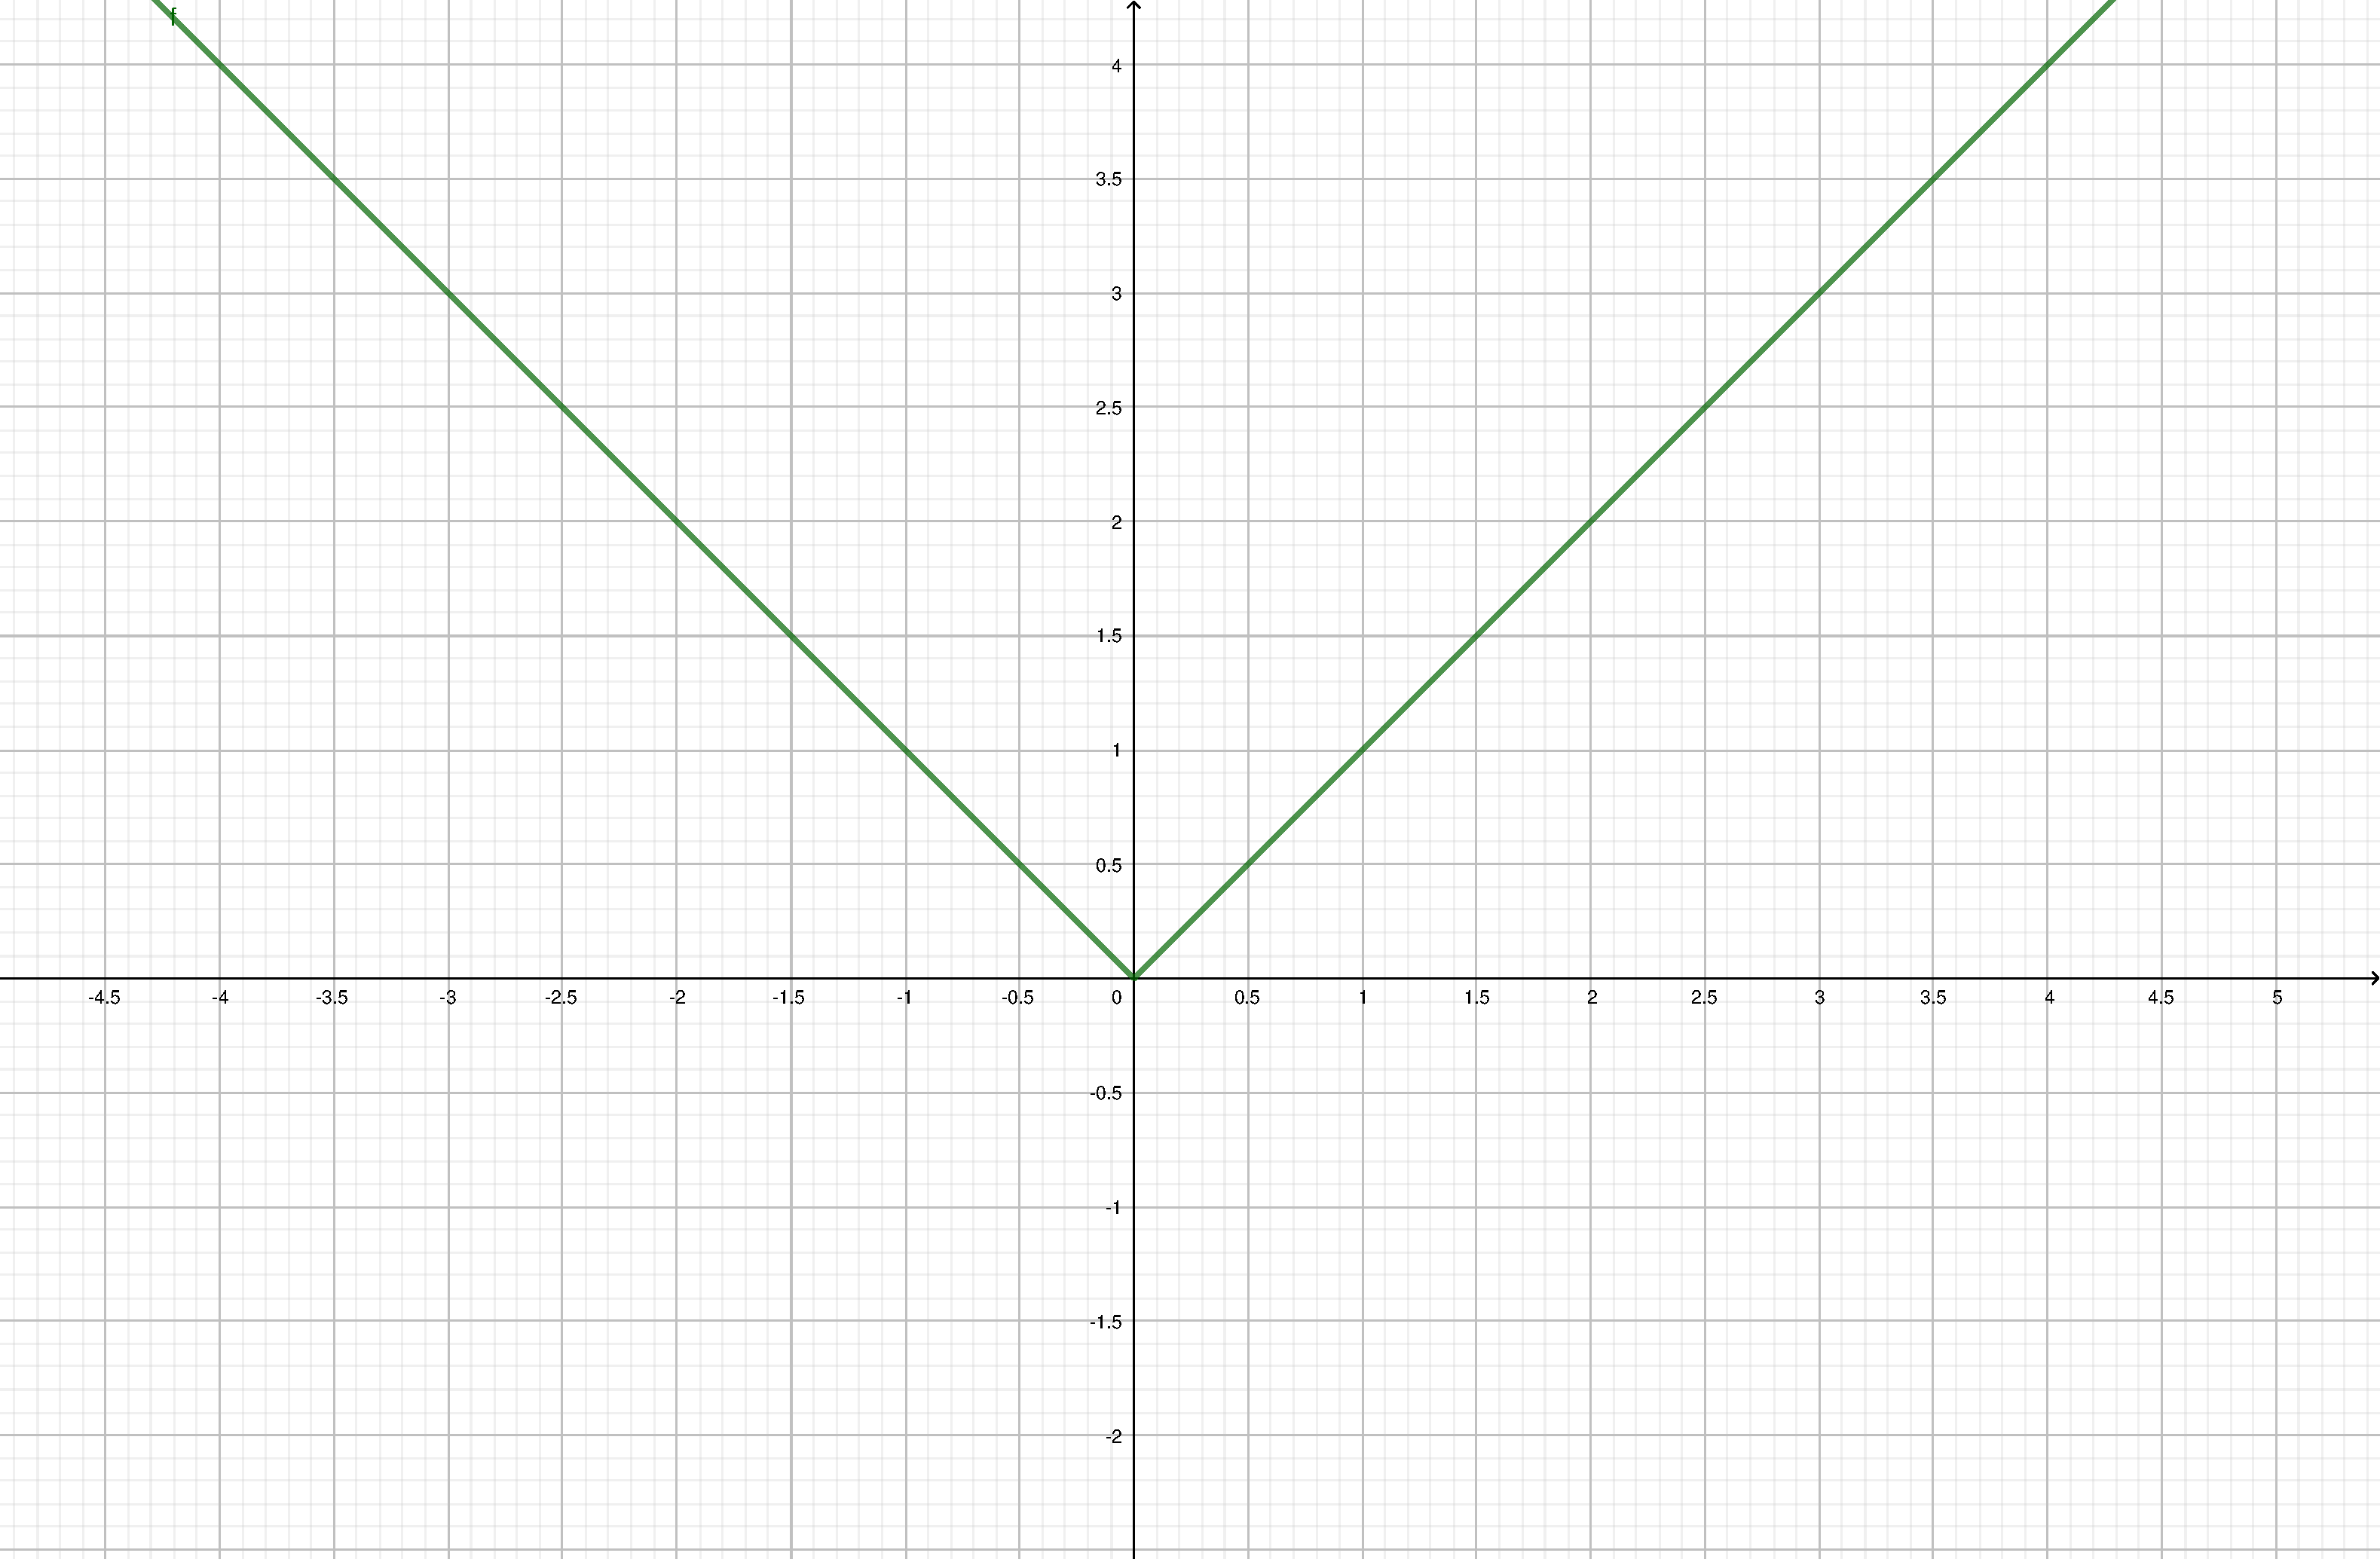
\includegraphics[height=8cm]{img/funzione valore assoluto.pdf}};
	\end{tikzpicture}
	\caption{Grafico di Funzione valore assoluto $y=|x|$ e quindi $f^,_+(0)=1\neq
	f^,_+=-1$}
\end{figure}
\subsubsection{Un altro esempio}
\begin{figure}[!ht]
	\centering
	\begin{tikzpicture}
		\node[] (pic) at (0,0) {\includegraphics[height=8cm]{img/esempio punto
		angoloso.pdf}};
	\end{tikzpicture}
	\caption{Grafico di Funzione $x=|x^2-1|$}
\end{figure}
\subsection{Punto cuspude}
Se $f^,_+(x)\neq f^,_-(x)$ sono $\infty$, $x_0$ si dece \colorbox{yellow}{punto
cuspide}; la retta tangente alla \textit{f(x)} nel punto di ascissa $x_0$ è
verticale.
\begin{figure}[!ht]
	\centering
	\begin{tikzpicture}
		\node[] (pic) at (0,0) {\includegraphics[height=8cm]{img/esempio punto
		cuspide.pdf}};
	\end{tikzpicture}
	\caption{Grafico di Funzione $f(x)=\frac{(x-3)^{\frac{2}{3}}}{2}$}
\end{figure}
\subsubsection{Punto di flesso a tangente verticale}
Se $f^,_+(x_0)=f^,_-(x_0)=\pm \infty$ sono $\infty$, $x_0$ si dice punto di
flesso a tangente verticale; la retta tangente alla $f(x)$ nel punto di ascissa
$x_0$ è verticale.
\subsection{Esempi di derivate}
\begin{multicols}{2}
	\begin{itemize}
		\item $D(x^n)=n*x^{n-1}$
		\item $D(\log_ax=\frac{1}{x}\log_a e)$
		\item $D(a^x)=a^x\ln a$
		\item $D(\sin x)=\cos x$
		\item $D(\cos x)=-\sin x$
		\item $D(k)=0$
		\item $D(\ln x)=\frac{1}{x}$
		\item $D(e^x)=e^x$
		\item $D(\tan x)=\frac{1}{\cos^2 x}=1+\tan^2x$
		\item $D(\arcsin x)=\frac{1}{\sqrt{1-x^2}}$
		\item $D(\arccos x)=-\frac{1}{\sqrt{1-x^2}}$
		\item $D(\arctan x)=\frac{1}{1+x^2}$
	\end{itemize}
\end{multicols}
\subsubsection{Qualche esercizio dimostrativo}
Utilizzando la definizione calcolare la derivata di
\begin{enumerate}
	\item $f(x)=k$\\
		$f^\prime(x)=\lim_{h\to 0}\frac{f(x+h)-f(x)}{h}=\lim_{h\to 0}\frac{k-k}{h}=0$
	\item $f(x)=e^x$\\
		$f^\prime(x)=\lim_{h\to 0}\frac{f(x+h)-f(x)}{h}=\lim_{h\to
		0}\frac{e^x(e^h-1)}{h}=e^x$
	\item $f(x)=\ln x$\\
		$f^\prime(x)=\lim_{h\to 0}\frac{f(x+h)-f(x)}{h}=\lim_{h\to
		0}\frac{\ln(x+h)\ln x}{h}=\frac{\ln(1+\frac{h}{x})}{h}=\frac{1}{x}$
	\item $f(x)=\cos x$\\
		$f^\prime(x)=\lim_{h\to 0}\frac{f(x+h)-f(x)}{h}=\lim_{h\to
		0}\frac{\cos(x+h)-\cos(x)}{h}=\lim_{h\to 0}\frac{\cos x*\cos h-\sin
		x*\sin h-\cos(x)}{h}=$\\$\lim_{h\to 0}\frac{\cos x (\cos h -
		1)}{h}-\frac{\sin x\sin h}{h}=-\sin x$
	\item $f(x)=\sin x$\\
		$f^\prime(x)=\lim_{h\to 0}\frac{f(x+h)-f(x)}{h}=\lim_{h\to
		0}\frac{\sin(x+h)-\sin(x)}{h}=\frac{\sin x \cos h +\sin h \cos x-\sin
		x}{h}=\lim_{h\to 0}\frac{\sin x(\cos h-1)}{h}+\lim_{h\to 0}\frac{\sin
		h\cos x}{h}=\cos x$
\end{enumerate}
\textit{Se f e g sono derivabile in x, allora sono derivabili in x anche la
somma, la differenza, il prodotto, il quoziente (con il denominatore$\neq 0$) e
si ha:}
\begin{enumerate}
	\item $(f\pm g)^\prime=f^\prime\pm g^\prime$
	\item $(f*g)^\prime=f^\prime*g+f*g^\prime$
	\item $(\frac{f}{g})^\prime=\frac{f^\prime*g-f*g^\prime}{g^2}, g\neq 0$
\end{enumerate}
\begin{itemize}
	\item \textit{Dimostriamo la 2)} $(f*g)^\prime=f^\prime*g+f*g^\prime$\\
		$(f*g)^\prime=\lim_{h\to 0}\frac{f(x+h)g(x+h)-f(x)g(x)}{h}=\lim_{h\to
0}\frac{f(x+h)g(x+h)\pm f(x)g(x+h)-f(x)g(x)}{h}=$\\
		$\lim_{h\to
0}\frac{g(x+h)[f(x+h)-f(x)]}{h}+\lim_{h\to 0}\frac{f(x)[f(x+h)-f(x)]}{h}$\\
Per ipotesi f e g sono derivabile, quindi continue in x, perciò:\\
$\lim_{h\to 0}g(x+h)=g(x),$
\begin{center}
	$(f*g)^\prime=...=f^\prime(x)*g(x)+f(x)*g^\prime(x)$
\end{center}
\item \textit{Dimostriamo la 3)}\\
	$(\frac{f}{g})^\prime=\frac{\frac{f(x+h)}{g(x+h)}-\frac{f(x)}{g(x)}}{h}=\frac{f(x+h)g(x)-f(x)g(x+h)}{g(x+h)g(x)*h}=\frac{f(x+h)g(x)-f(x)g(x+h)\pm
		f(x)g(x)}{g(x+h)g(x)*h}$\\
		$\frac{[f(x+h)-f(x)]g(x)-f(x)[g(x+h)-g(x)]}{g(x+h)g(x)*h}=\frac{\frac{[f(x+h)-f(x)]g(x)}{h}-\frac{f(x)[g(x+h)-g(x)]}{h}}{g(x+h)g(x)*h}=$\\$\frac{f^,(x)g(x)-f(x)g^,(x)}{g(x+h)g(x)*h}=\frac{f^,(x)g(x)-f(x)g^,(x)}{[g(x)]^2*h}$

\end{itemize}
\subsubsection{Esercizio}
\begin{itemize}
	\item \textit{Calcolare la derivata di $f(x)=\sin x \ln x$}\\
		$f^\prime(x)=\cos x \ln x+\frac{sin x}{x}$
	\item \textit{Scrivere l'equazione della retta tangente alla curva di eq
		$f(x)=2e^x\sqrt[3]{x}$ nel punto di ascissa x=1}\\
		$f^\prime(x)=2e^x\sqrt[3]{x}+2\frac{e^x}{3\sqrt[3]{x^2}}$
\end{itemize}
\subsection{Teorema di derivazione della funzione composta}
\textit{Sia g(x) una funzione derivabile in x, e se f(x) è una funzione
derivabile nel punto g(x), allora la funzione composta f(g(x)) è derivabile in
x, e si ha:}
\begin{center}
	$[f(g(x))]^\prime=f^\prime(g(x))*g^\prime(x)$
\end{center}
Dimostrazione. Se $h\neq 0$ si ha $\lim_{h\to
0}\frac{f(g(x+h))-f(g(x))}{h}=\lim_{h\to
0}\frac{f(g(x+h))-f(g(x))}{h}*\frac{g(x+h)-g(x)}{h}=f^\prime(g(x))*g^\prime(x)$
\textit{in quanto se $h\to 0$ allora $k\to 0$ con $k=g(x+h)-g(x)$, essendo
g(x) continua in x. Se h=0, il teorema continua a valere.}
\subsubsection{Esercizio}
\begin{enumerate}
	\item Calcolare la derivata di $f(x)=\ln(\sin x)$.\\
		$f^\prime (x)=\frac{\cos x}{\sin x}=\cot{x}$
	\item Calcolare la derivata di $f(x)=e^{\sqrt{2x^3+x}}.$\\
		$f^\prime (x)=e^{\sqrt{x^3+x}}\frac{6x^2+1}{2\sqrt{2x^3+x}}$
	\item Calcolare la derivata di $f(x)=\sin(\ln x)$\\
		$f^\prime (x)=\frac{\cos(\ln x)}{x}$
\end{enumerate}
Scrivere l'equazione della retta alla curva di equazione $f(x)=(xe^{2x}-1)^3$
nel punto di ascissa x=0, L'eq. Retta tangente a $f(x)$ in $x=x_0:
y=f^\prime(x_0)(x-x_0)+f(x_0)$\\
Per noi $x_0=0$\\
$f^\prime(x)=3(xe^{2x}-1)^2(e^{3x}+xe^{2x})\Rightarrow f^\prime (0)=3$\\
$f(0)=-1$\\
Quindi l'equazione è: $y=3x-1$
\subsection{Teorema di derivazione della funzione inversa}
\textit{Sia f(x) una funzione continua e strettamente monotona in [a,b]. Se f è
derivabile in $x_0\in(a,b)$ e se allora anche la funzione inversa di $f^{-1}$ è
derivabile nel punto $y_0=f(x_0)$, e la derivata vale:}
\begin{center}
	$[f^{-1}(y_0)]^\prime=\frac{1}{f^\prime(x_0)}$
\end{center}
Dimostrazione. Si ha
$\frac{f^{-1}(y_0+k)-f^{-1}(y_0))}{k}=\frac{h}{f(x_0+h)-f(x_0}$
% grafici
Se $k\to 0$ anche $h\to0$ in quanto $f^\prime$ è continua
\subsection{Esercizio}
Utilizzando il teorema di derivazione della funzione inversa, dimostrare che:
\begin{center}
	$D[\arcsin(y)]=\frac{1}{\sqrt{1-y^2}}$
\end{center}
$x=\arcsin(y)$ è la funzione inversa di $y=\sin(x)$ quest'ultima è invertibile
per $x\in [-\frac{\pi}{2};\frac{\pi}{2}]$. Applichiamo il teorema della
funzione inversa, $f^{-1}(y)=\frac{1}{f^\prime(x)}$\\
\begin{tabular}{|l|}
	\hline
	$[\arcsin(y)]^\prime=\frac{1}{[\sin(x)]^\prime}=\frac{1}{\cos(x)}$\\\hline
\end{tabular}\\
Ma sappiamo che: $\cos(x)=\sqrt{1-\sin^2x}$\\
\begin{tabular}{|l|}
	\hline
	$[\arcsin(y)]^\prime=\frac{1}{\sqrt{1-\sin^2x}}=\frac{1}{\sqrt{1-y^2}}$\\\hline
\end{tabular}
\subsection{Esercizio}
Calcolare la derivata della funzione $y=e^x$ vista come funzione inversa di
$f(x)=\ln x$. Per $x>0$, si ha $x=f^{-1}(y)=e^y$
$f(x)=\ln x\Rightarrow f^\prime(x)=\frac{1}{x}$ Perciò, per il teorema della
derivata della funzione inversa si ha
$(f^{-1}(y))^\prime=\frac{1}{f^\prime(x)}\Rightarrow (e^y)^\prime=x=e^y$.
Quindi $(e^x)^\prime=e^x$
\subsection{Esercizio}
Utilizzando il teorema di derivazione della funzione inversa, dimostrare che
$(\arctan x)^\prime=\frac{1}{1+x^2}$. Sia $f(x)=\tan x$, in
$x\in[-\frac{\pi}{2},\frac{\pi}{2}]$ si ha $x=f^{-1}(x)=\arctan y$\\
$f(x)=\tan x\Rightarrow f^\prime(x)=1+\tan^2x$. Perciò, per il teorema della
derivata della funzione inversa si ha
$(f^{-1}(y))^\prime=\frac{1}{f^\prime(x)}\Rightarrow (\arctan
y)^\prime=\frac{1}{1+\tan^2 x}=\frac{1}{1+y^2}$
\section{Massimo e minimo assoluto}
Sia $f:[a,b]\to R$, si dice M è \texttt{massimo assoluto} (o globale) di
\textit{f} in $[a, b]$ e $x_0\in[a, b]$ è un punto di massimo se
\begin{center}
	$f(x_0)=M\geq f(x),\forall x \in [a, b]$
\end{center}
\paragraph{in modo analogo:}
Si dice che m è un \texttt{minimo assoluto} (o globale) di
\textit{f} in $[a, b]$ e $x_1\in[a, b]$ è punto di minimo se 
\begin{center}
	$f(x_1)=M\leq f(x),\forall x \in [a, b]$
\end{center}
\section{Massimo e minimo relativo (o estremi locali)}
Sia $f:[a,b]\to R$, si dice che $x_0\in[a, b]$ è un punto di \texttt{massimo
relativo} (o locale) per $f(x)$ se $\exists I (x_0,\delta)$:
\begin{center}
	$f(x_0)\geq f(x),\forall x \in I (x_0,\delta)$
\end{center}
\paragraph{In modo analogo:}
si dice che $x_0\in[a, b]$ è un punto di \texttt{minimo relativo} (o locale)
per $f(x)$ se $\exists I (x_0,\delta)$:
\begin{center}
	$f(x_0)\leq f(x),\forall x \in I (x_0,\delta)$
\end{center}
\subsection{Punti Stazionari}
\textit{I punti in cui f(x) ha derivata nulla ($f^\prime=0$) Si dice punti
stazionari o critici.}
\section{Teorema di Fermat}
\textit{Sia $f(x)$ definita in [a,b] e derivabile in $x_0\in(a, b)$. Se $x_0$ è
un punto di estremo locale allora}
\begin{center}
	$f^\prime (x_0)=0$
\end{center}
\paragraph{Dimostrazione} Sia $x_0$ un punto di massimo relativo, cioè $\exists
I (x_0,\delta)$: $f(x_0)\leq f(x_0+h), \forall h: |h|<\delta$ si ha:
$\frac{f(x_0+h)+f(x_0)}{h}\begin{cases}
	\leq 0 & \text{ se } 0<h<\delta\\
	\geq 0 & \text{ se } -\delta<h<0 
\end{cases}$ e 
\begin{itemize}
	\item $\lim_{h\to 0^+}\frac{f(x_0+h)-f(x_0)}{h}=f^\prime_+\leq 0$
	\item $\lim_{h\to 0^-}\frac{f(x_0+h)-f(x_0)}{h}=f^\prime_-\geq 0$
\end{itemize}
Ma essendo $f(x)$ derivabile in $x_0$:
\begin{center}
	$f^\prime_+(x_0)=f^\prime_-(x_0)\Rightarrow f^\prime=0$
\end{center}
Se $x_0=a$ allora $0<h<\delta$ e se $x_0$ è un punto di \texttt{massimo 
relativo} si ha $\lim_{h\to 0^+}\frac{f(a+h)-f(x)}{h}=f^\prime(a)\leq 0$.
Mentre, se parliamo del \texttt{minimo relativo} in $x_0=a$: 
$\lim_{h\to 0^-}\frac{f(a+h)-f(x)}{h}=f^\prime(a)\leq 0$ In modo analogo: se
$x_0=b$ è punto di \texttt{massimo relativo} (con $-\delta<h<0$) allora
$f^\prime(b)\geq 0$, se invece $x_0=b$ è un punto di \texttt{minimo relativo},
allora $f^\prime(b)\leq 0$
\section{Teorema di Rolle}
Sia $f:[a,b]\to R$.
\begin{enumerate}
	\item \textit{f è continua in $[a,b]$},
	\item \textit{f è derivabile in $(a,b)_{f(a)=f(b)}$}
	\item $f(a)=f(b)$
\end{enumerate}
Allora $\exists x_0 \in (a,b):f^\prime(x_0)=0$ Per il Teorema di Rolle esistono
almeno un punto a tangente orizzontale.
\subsection{Dimostrazione}
Per il Teorema di Weiestrass, $f$ ha massimo e minimo assoluti in $[a,b]$
($x_1,x_2\in[a,b]$):
\begin{center}
	$f(x_1)\leq f(x)\leq f(x_2).$
\end{center}
\textit{Se uno dei due è interno ad $[a,b]$, per esempio $x_1$ allora per il
Teorema di Fermat $f^\prime(x_1)=0$. Se invece nessuno dei due è interno ad
$[a,b]$ per esempio $x_1=a, \text{ } x_2=b$. Dall'ipotesi $f(a)=f(b)$ si ottiene
minimo=massimo, cioè $f(x)$ è costante $\forall x \in[a,b]$ e quindi
$f^\prime(x)=0\text{ } \forall x \in [a,b]$}.
\subsection{Esercizio dimostrativo}
\subsubsection{Testo}
Dire se la funzione $f(x)=e^{x^2-1}$ soddisfa il teorema di Rolle
nell'intervallo $[-1,1]$ e in caso affermativo calcolare il punto (o i punto
del Teorema.)
\subsubsection{Soluzione}
Sono verificate tutte le ipotesi del teorema di Rolle, infatti:
\begin{enumerate}
	\item $f(x)=e^{x^2-1}$ è continua in tutte R e quindi anche in $[-1,1]$
	\item f(x) è derivabile in tutto R, quindi anche in (-1,1),
	\item $f(-1)=f(1)$
\end{enumerate}
Allora $\forall x_0 \in (-1,1):f^\prime(x_0)=0$\\
$x_0$ Si ricava facendo il calcolo: $f^\prime (x_0)=0$, cioè
$2xe^{x^2-1}=0\Rightarrow x_0=0$
\subsection{Esercizio dimostrativo}
\subsubsection{Testo}
Dire se la funzione $f(x)=\ln|x|$ soddisfa il teorema di Rolle nell'intervallo
[-e,e].
\subsubsection{Soluzione}
Il teorema di Rolle non è applicabile perché $f(x)=\ln|x|$ non è definita in
$x=0$, quindi non è né continua né definita in $x=0$ e perciò non soddisfa
tutte le ipotesi del teorema.
\section{Teorema di Lagrange ({\em o del valor medio})}
Sia $f:[a,b]\to R$.
\begin{enumerate}
	\item \textit{f è continua in $[a,b]$},
	\item \textit{f è derivabile in $(a,b)$},
\end{enumerate}
Allora $\forall x_0\in(a,b):f^\prime (x_0)=\frac{f(b)-f(a)}{b-a}$\\
\textit{Per il Teorema di Lagrange $\exists$ almeno un punto ($x_0,f(x_0)$) sul
grafico di f(x) in cui la retta tangente \textbf{t} è parallela alla retta
\textbf{r} secante la curva in $(a,f(a))$ e $b,f(b)$}.
\subsection{Dimostrazione}
Si considera la funzione ausiliaria 
\begin{center}
	$g(x)=f(x)-[\overset{\text{equazione di
	r}}{f(a)+\frac{f(b)-f(a)}{b-a}(x-a)}]$
\end{center}
Per g(x) vale il Teorema di Rolle, infatti:
\begin{enumerate}
	\item \textit{g(x) è continua in $[a,b]$ perché lo è f(x) (l'altro pezzo è
		lineare)};
	\item \textit{g(x) è derivabile in $(a,b)$ perché f(x) (l'altro pezzo è
		lineare)};
	\item $g(a)=g(b)=0$.
\end{enumerate}
\begin{itemize}
	\item $\Rightarrow x_0:g^\prime (x)=0$
	\item $g^\prime (x_0)=f^\prime(x_0)-\frac{f(b)-f(a)}{b-a}=0$
	\item $\Rightarrow f^\prime(x_0)=\frac{f(b)-f(a)}{b-a}$
\end{itemize}
\subsection{Esempio}
$f(x)=x^2 \text{ in } [a,b]$, per il Teorema di Lagrange $\forall x_0 \in
[a,b]$:
\begin{center}
	$\frac{b^2-a^2}{b-a}=2x_0\Rightarrow x_0=\frac{b+a}{2}$ Media aritmetica di
	a e b
\end{center}
\subsection{Esercizio dimostrativo}
\subsubsection{Testo}
\textit{Dire se è applicabile in Teorema di Lagrange alla funzione
$f(x)=\arcsin x$ nell'intervallo $[-1,1]$ e in caso affermativo calcolare i
punti teorema.}
\subsubsection{Soluzione}
La funzione data soddisfa tutte le ipotesi del teorema di Lagrange, infatti:
\begin{enumerate}
	\item $f$ è continua in [-1,1] (è il suo campo di esistenza),
	\item $f$ è derivabile in (-1,1)\\
		Allora $\forall x_0\in (-1.1):f^\prime
		(x_0)=\frac{f(1)-f(-1)}{2}\Rightarrow
		\frac{1}{\sqrt{1-x^2_0}}=\frac{\pi}{2}\Rightarrow
		x_0=\pm\frac{\sqrt{\pi^2-4}}{\pi}$
\end{enumerate}
\subsection{Esercizio dimostrativo}
\subsubsection{Testo}
Determinare un intervallo in cui è applicabile il Teorema di Lagrange alla
funzione $f(x)=|x-\frac{1}{x}|$.
\subsubsection{Soluzione}
\begin{enumerate}
	\item La funzione data è contenuta nel suo campo di esistenza cioè
		nell'insieme: $A=\{x \in R: x\neg 0\}$
	\item f è derivabile nell'insieme $B=\{x\in R: x\neq 0,\pm 1\}$ con
		derivata: $f^\prime(x)=|\frac{x^2-1}{x}|\frac{x^2+1}{x(x^2-1)}$
\end{enumerate}
Perciò un intervallo in cui $f$ soddisfa il teorema di Lagrange, è un qualunque
intervallo $[a,b]$ che contiene $x=0$ e tale che punti $x=-1$ non siano interni
ad esso (potrebbero stare agli estremi)\\
Per esempio: $[1,2]$ (f è continua in [1,2] e derivabile in (1,2), da notare
che è derivabile anche in $x=2$ ma non serve\dots) oppure $[-4,-3]$. etc\dots

